\documentclass[
notumble,
%%nofoldmark,
%%dvipdfm,
%%portrait,
% titlepage,
% nocombine,
%%a3paper,
%%debug,
%%nospecialtricks,
%%draft,
]{leaflet}
%\documentclass[a4paper,10pt,titlepage]{leaflet}

\usepackage[utf8]{inputenc}

% Language
\usepackage{comment}
\includecomment{german}
%\excludecomment{german}
% \includecomment{english}
\excludecomment{english}

\begin{german}
\usepackage[ngerman]{babel}
\end{german}
\begin{english}
\usepackage[english]{babel} 
\end{english}



\usepackage[T1]{fontenc}
\usepackage{graphicx}
\usepackage{shortvrb}
\usepackage{textcomp}
\usepackage{mathptmx}
%\usepackage[scaled=0.9]{helvet}
%\usepackage{url}
\usepackage{hyperref}
\usepackage{blindtext}
\usepackage{graphicx}
\usepackage[dvipsnames,usenames]{color}
\newcommand{\okf}{Open Knowledge Foundation}


\definecolor{LIGHTGRAY}{gray}{.9}
%\definecolor{HOHBLUE}{rgb}{0,63,117}
\definecolor{HOHBLUE}{cmyk}{1,0.5,0,0.45}
% \definecolor{LDGREEN}{cmyk}{0.8625,0,0.1687,0.3725} %#16A085; Red Green Blue RGB Decimal Value 22 160 133 Cyan Magenta Yellow blacK  86.25  0  16.87  37.25
% color from svg HEX-DEC: 1A=26 BC=188 9C=156
\definecolor{LDGREEN}{rgb}{0.101,0.737,0.611}
%\definecolor{HOBLUELIGHT}{rgb}{}

%\CutLine*{1}% Dotted line without scissors
\CutLine*{6}% Dotted line without scissors
%\CutLine{6}%  Dotted line with scissors

% \AddToBackground{1}{%  Background of a small page
%   \put(0,0){
\includegraphics[width=\textwidth]{images/logo_luftdaten_info}}}
%   \textcolor{LDGREEN}{\rule{\paperwidth}{\paperheight}}}}
%\AddToBackground{1}{%  Background of a small page
%  \put(0,0){\textcolor{LIGHTGRAY}{\rule{\paperwidth}{\paperheight}}}}
% \AddToBackground*{2}{% Background of a large page
%   \put(\LenToUnit{.35\paperwidth},\LenToUnit{.4\paperheight}){%
%     \makebox(0,0)[c]{%
%       \resizebox{.7\paperwidth}{!}{
%         %\textsf{\textbf{\textcolor{LIGHTGRAY}{SENGIS}}}
% 	
\includegraphics[width=\textwidth]{../logo/logo_luftdaten_info}
% }}}}
\begin{document}
\color{LDGREEN}
\begin{center}

\includegraphics[width=\textwidth]{images/logo_luftdaten_info}
\\[2em]
\sffamily
\huge
Feinstaub selbst messen
\\[1em]
Luftdaten.info
\\[1em]
Open Knowledge Foundation 
\\
Stuttgart
\normalsize 
\normalfont
\end{center}
\color{black}

\newpage
% \begin{center}
% \includegraphics[width=0.5\textwidth]{uni-logo_zeichen_schwarz_bb}
% \end{center}


\begin{quote}
„Mit einem einfachen Einplatinenrechner in sehr kleiner Abmessung und einem Schadstoffsensor aus einer Klimaanlage wollen das OKLab Stuttgart die regelmäßig unter zu hohen Feinstaubwerten leidende Stadt Stuttgart mit einem Feinstaubmessgerätenetz überziehen.“
\end{quote}
\raggedright{Feinstaubbelastung selber messen und \#bcnue8, Podcast: NightShift, von Michael Fohrn, 15. März 2016}


\section{OK LAB STUTTGART}

Das OK Lab Stuttgart ist Teil des Programms Code for Germany der Open Knowledge Foundation Germany. Ziel des Programms ist es, Entwicklungen im Bereich Transparenz, Open Data und Citizen Science zu fördern. Regionale Gruppen bestehend aus Designern, Entwicklerinnen, Journalisten und Anderen, treffen sich regelmäßig in Labs. Sie entwickeln Apps, die informieren, die Gesellschaft positiv gestalten und unterstützen und die Arbeit von Verwaltungen und Behörden transparenter machen.

\begin{figure}
\noindent
\includegraphics[width=\textwidth]{images/CFG_logo}\\
\noindent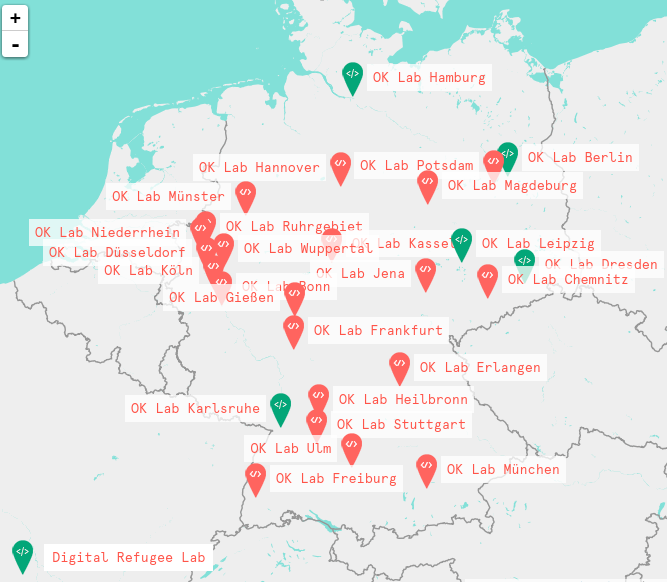
\includegraphics[width=\textwidth]{images/codefordemap}
\end{figure}

Wir sind mittlerweile ein fester Stamm von 10 Leuten und arbeiten in verschiedenen Gruppen an Projekten rund um Transparenz, Open Data, Civic Tech, Datenvisualisierung und Citizen Science. Wir kommen aus ganz verschiedenen Bereichen und setzen uns zusammen aus DesignerInnen, EntwicklerInnen, JournalistInnen, ProgrammiererInnen und Anderen. Entsprechend behandeln auch die Projekte, an denen wir arbeiten, ganz unterschiedliche Themen. Wir entwickeln Apps, die informieren, die Gesellschaft positiv gestalten und unterstützen und die Arbeit von Verwaltungen und Behörden transparenter machen.

Wir treffen uns \textit{jeden 4. Dienstag um 18.30 Uhr in der Stadtbibliothek} am Mailänder Platz. Dort können Interessierte ihre Ideen mitbringen und sich vorstellen und wir zeigen, woran wir gerade arbeiten. Wenn Du Lust hast, Dir unser Lab anzuschauen, komm einfach zu einer der Vorstellungsrunden vorbei.

An \textit{jedem 2. Dienstag im Monat treffen wir uns im Shackspace} in Stuttgart Wangen und arbeiten an unserer Hardware weiter. Im Moment beschäftigen wir uns mit Feinstaub-Sensoren.

Hack your City Das OK Lab Stuttgart arbeitet 2015 schwerpunktmäßig an Citizen Science Projekten. Im Rahmen des Projekts Hack your City findet am 13. und 14. Juni dazu ein Citizen Science Hackday in Karlsruhe statt, bei dem auch das Feinstaub-Projekt luftdaten.info vorgestellt wird. Hack your City ist ein Projekt im Rahmen des Wissenschaftsjahr 2015 - Zukunftsstadt. Mehr Informationen findest Du hier: hackyourcity.de

Weitere Ideen zu Transparenz, Open Data, Civic Tech, Datenvisualisierung und Citizen Science sind immer willkommen.


% Meetup
% Twitter
% Etherpad
% KONTAKT

% Jan A. Lutz
% PRESSE

\section{LUFTDATEN SELBER MESSEN}

Das OK Lab Stuttgart widmet sich zur Zeit der Feinstaubmessung. Selbst gebaute Feinstaubmessgeräte werden an Paten im gesamten Stuttgarter Raum vergeben. Die gesammelten Daten werden in Echtzeit auf einer Webseite visualisiert. So wird Feinstaub sichtbar. Weitere Ideen sind immer willkommen.
Spenden lagen zwischen 20 und 50 Euro, Paten bringen ein Feinstaub-Messgerät außen an ihrer Wohnung/Haus an und verbinden es mit einem W-Lan Anschluss.

% Es gab eine erfolgreiche Spendenaktion.
Der reine Materialwert eines Feinstaub Messgeräts liegt bei +/- 30,00 €. 
% Deshalb gilt als Richtwert für die Spende für ein Messgerät dieser Betrag. Gerne kann mehr oder weniger gespendet werden.
% Mehr Infos zum Spenden gibt's in der Projektübersicht.
% 
% Die Spendenaktion war erfolgreich. 
In Kürze werden wir mit dem Bau der Sensoren, die aus der Spendenaktion finanziert wurde, beginnen. 
Dazu wird es Workshops für kleine Gruppen geben. Bleibe auf dem Laufenden und trage dich in den Newsletter ein.
Es kann gerne auch noch weiter gespendet werden.

Willst du zum Feinstaub-Messprojekt auf dem Laufenden gehalten werden oder interessierst du dich für eine Patenschaft für eines der Messgeräte?
Dann trag dich mit deiner E-Mail Adresse auf der Webseite ein:

\href{http://luftdaten.info/}{luftdaten.info}

Das OK Lab Stuttgart trifft sich jeden:
\begin{description}
 \item [2. Dienstag] im Monat im shackspace in Stuttgart Wangen.
 \item [4. Dienstag] im Monat in der Stadtbibliothek am Mailänderplatz.
\end{description}

Interessierte können gerne dazu kommen.

\section{Feinstaub Karte}
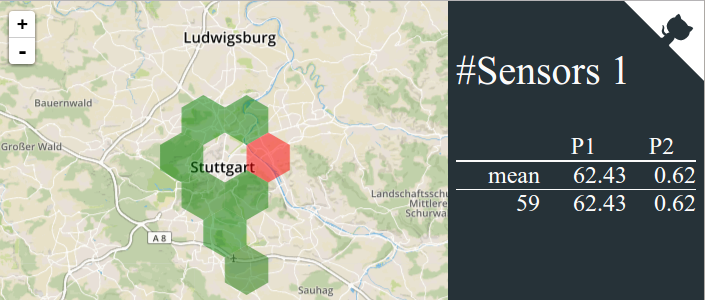
\includegraphics[width=\textwidth]{images/feinstaubmap}

\newpage 
\section{Die Hardware}

Für eine Station benötigte Bauteile:
\begin{itemize}
\item ESP8266 (WLAN, Prozessor) \\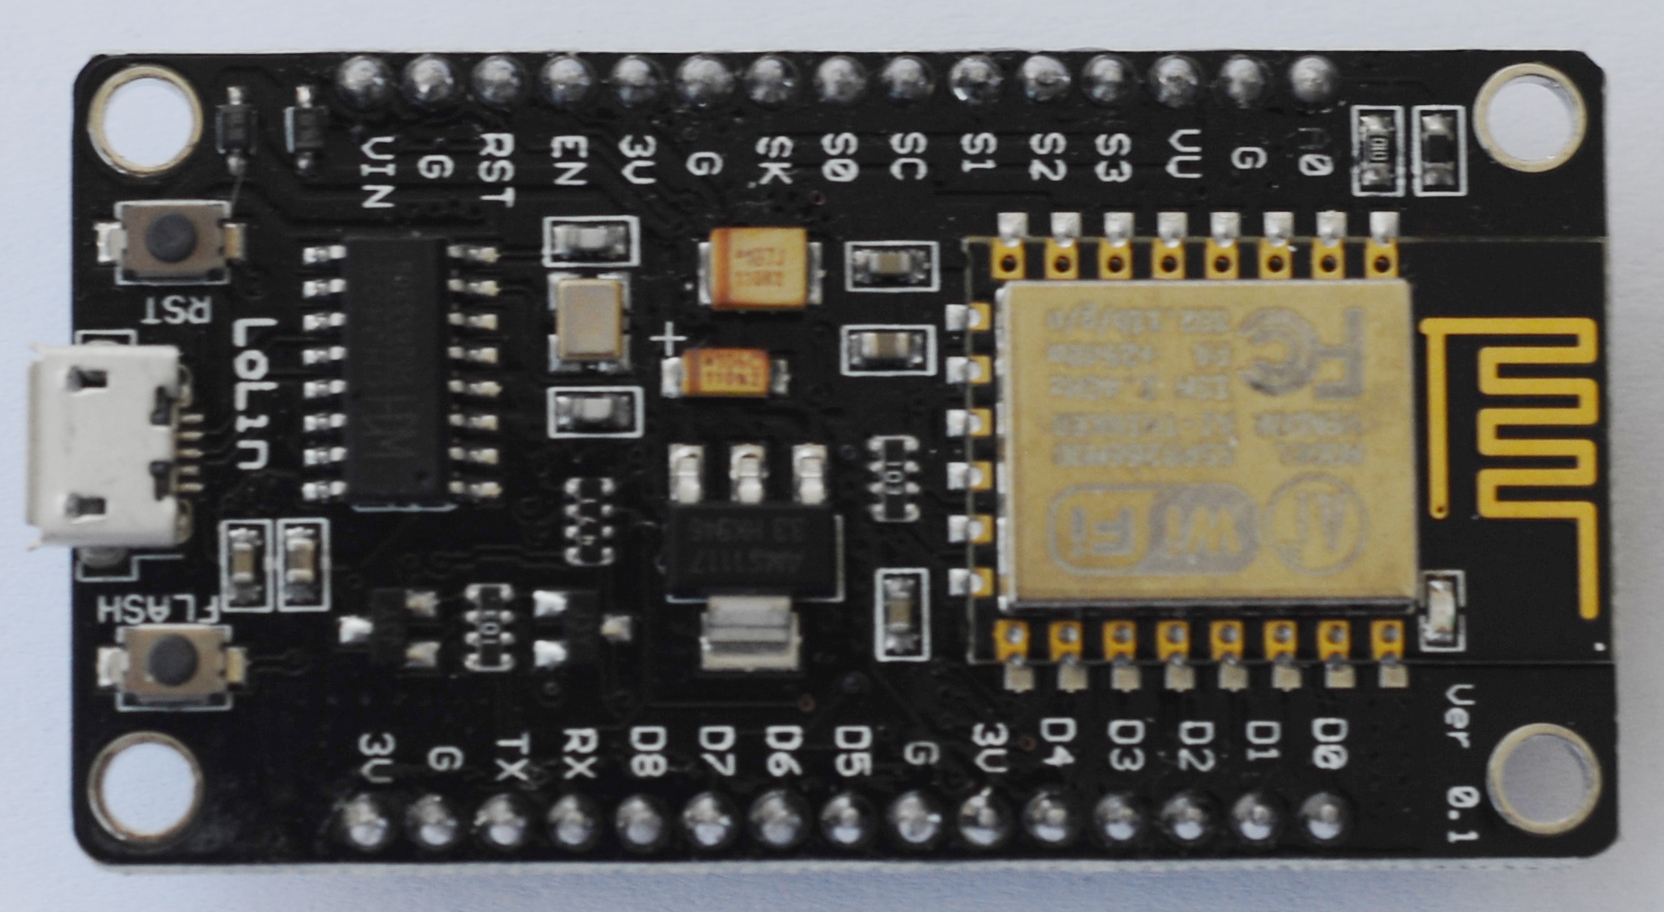
\includegraphics[width=0.49\textwidth]{images/sensor/esp8266.jpg} 
% \item PPD42NS (Feinstaub messen) \\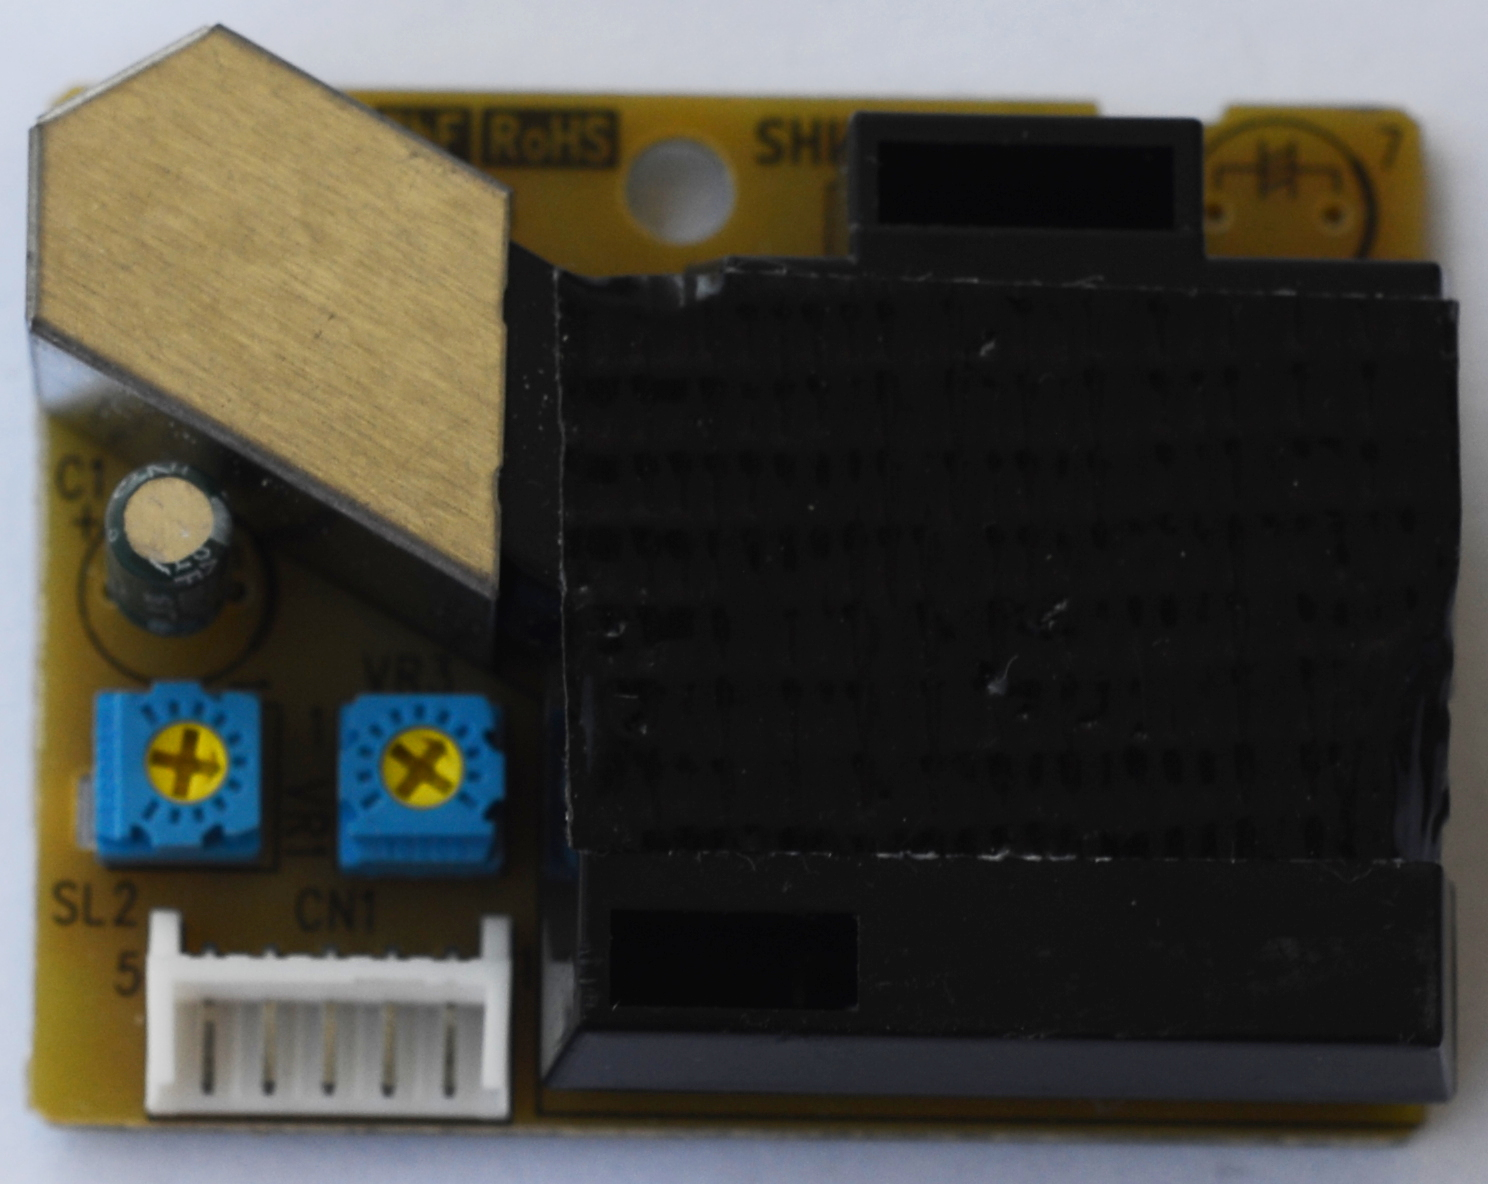
\includegraphics[width=0.49\textwidth]{images/sensor/ppd.jpg} 
\item SDS011 (Feinstaub messen), ersetzt PPD42NS \\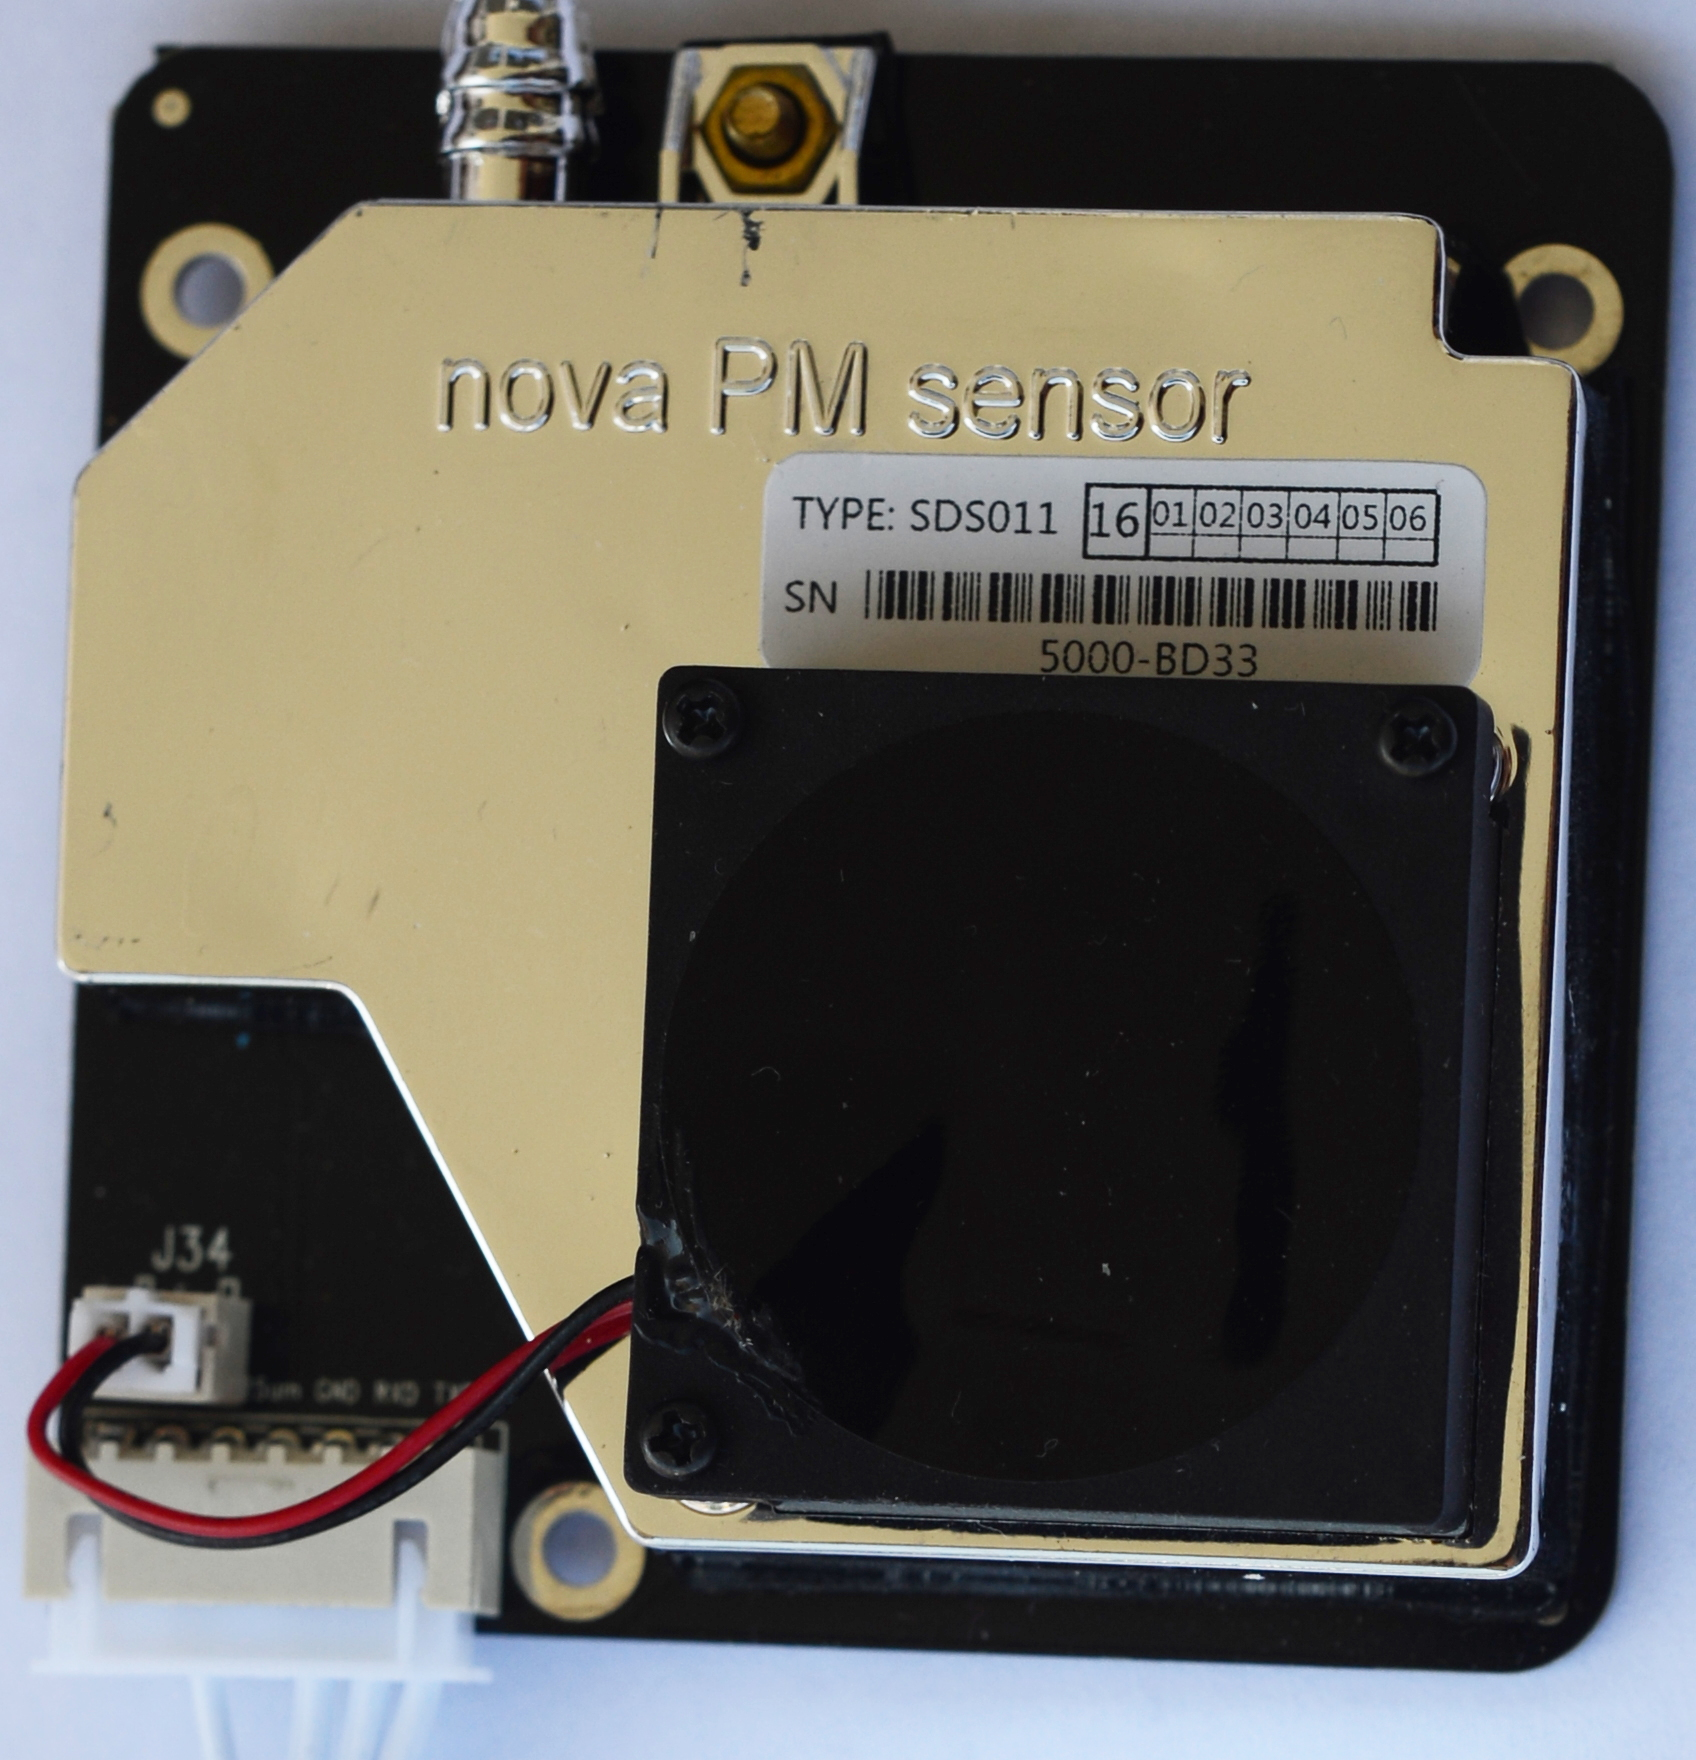
\includegraphics[width=0.49\textwidth]{images/sensor/sds011.jpg} 
\item DHT22 (Temperatur \& Luftfeuchtigkeit)\\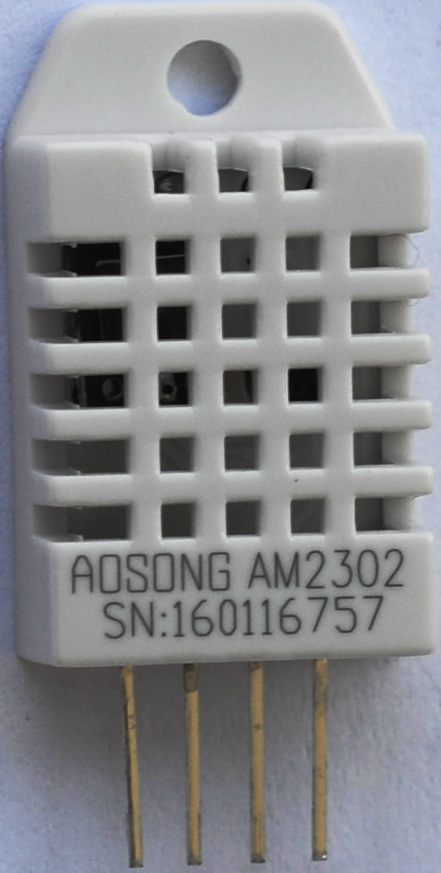
\includegraphics[width=0.19\textwidth,angle=90]{images/sensor/dht22.jpg}
\item Abflussröhren zur Außenmontage \\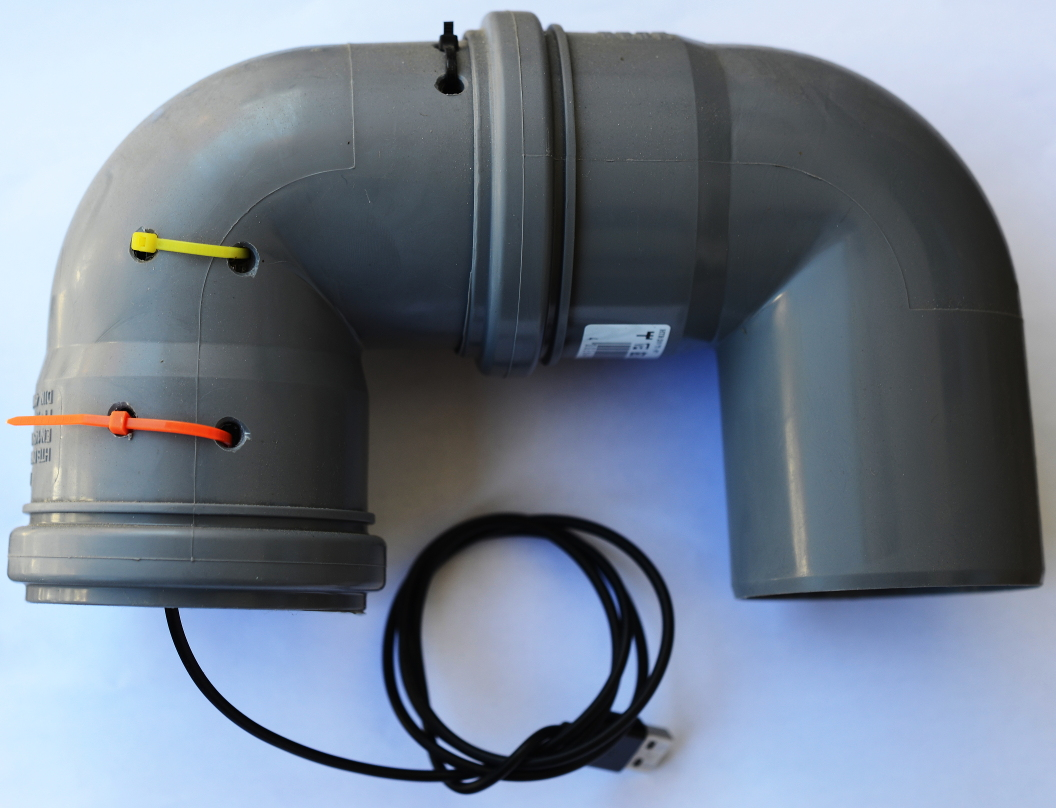
\includegraphics[width=0.49\textwidth]{images/sensor/roehren.jpg} 
\item Stromversorgung (MicroUSB-Netzteil oder Akku) \\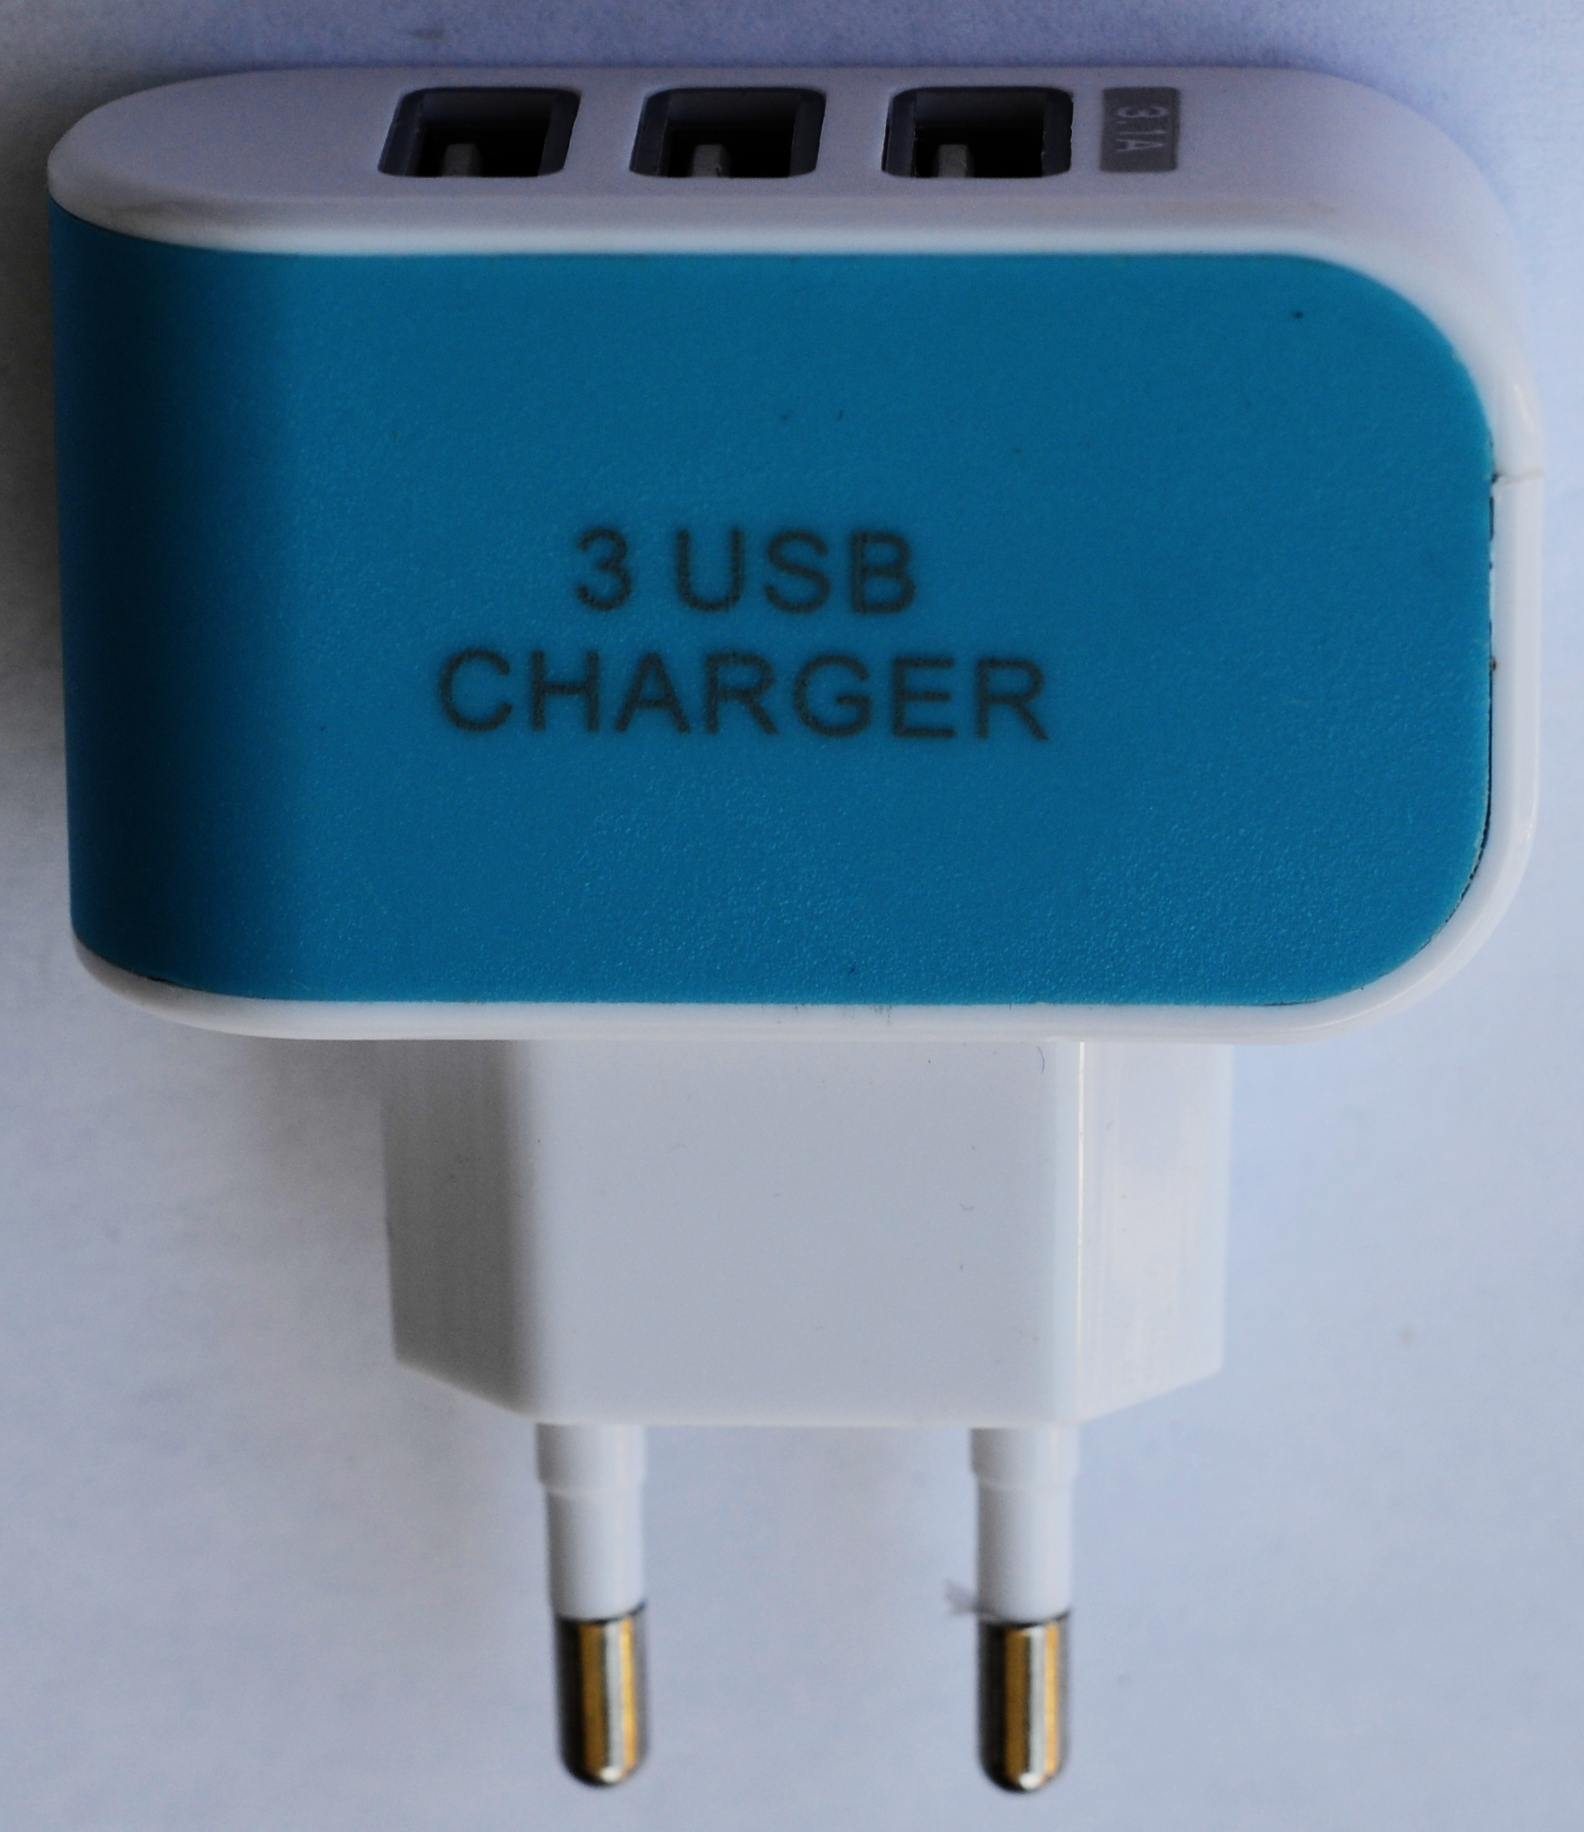
\includegraphics[width=0.49\textwidth]{images/sensor/usbcharger.jpg}
\item Kleinkram (Kabel, LED, \dots) \\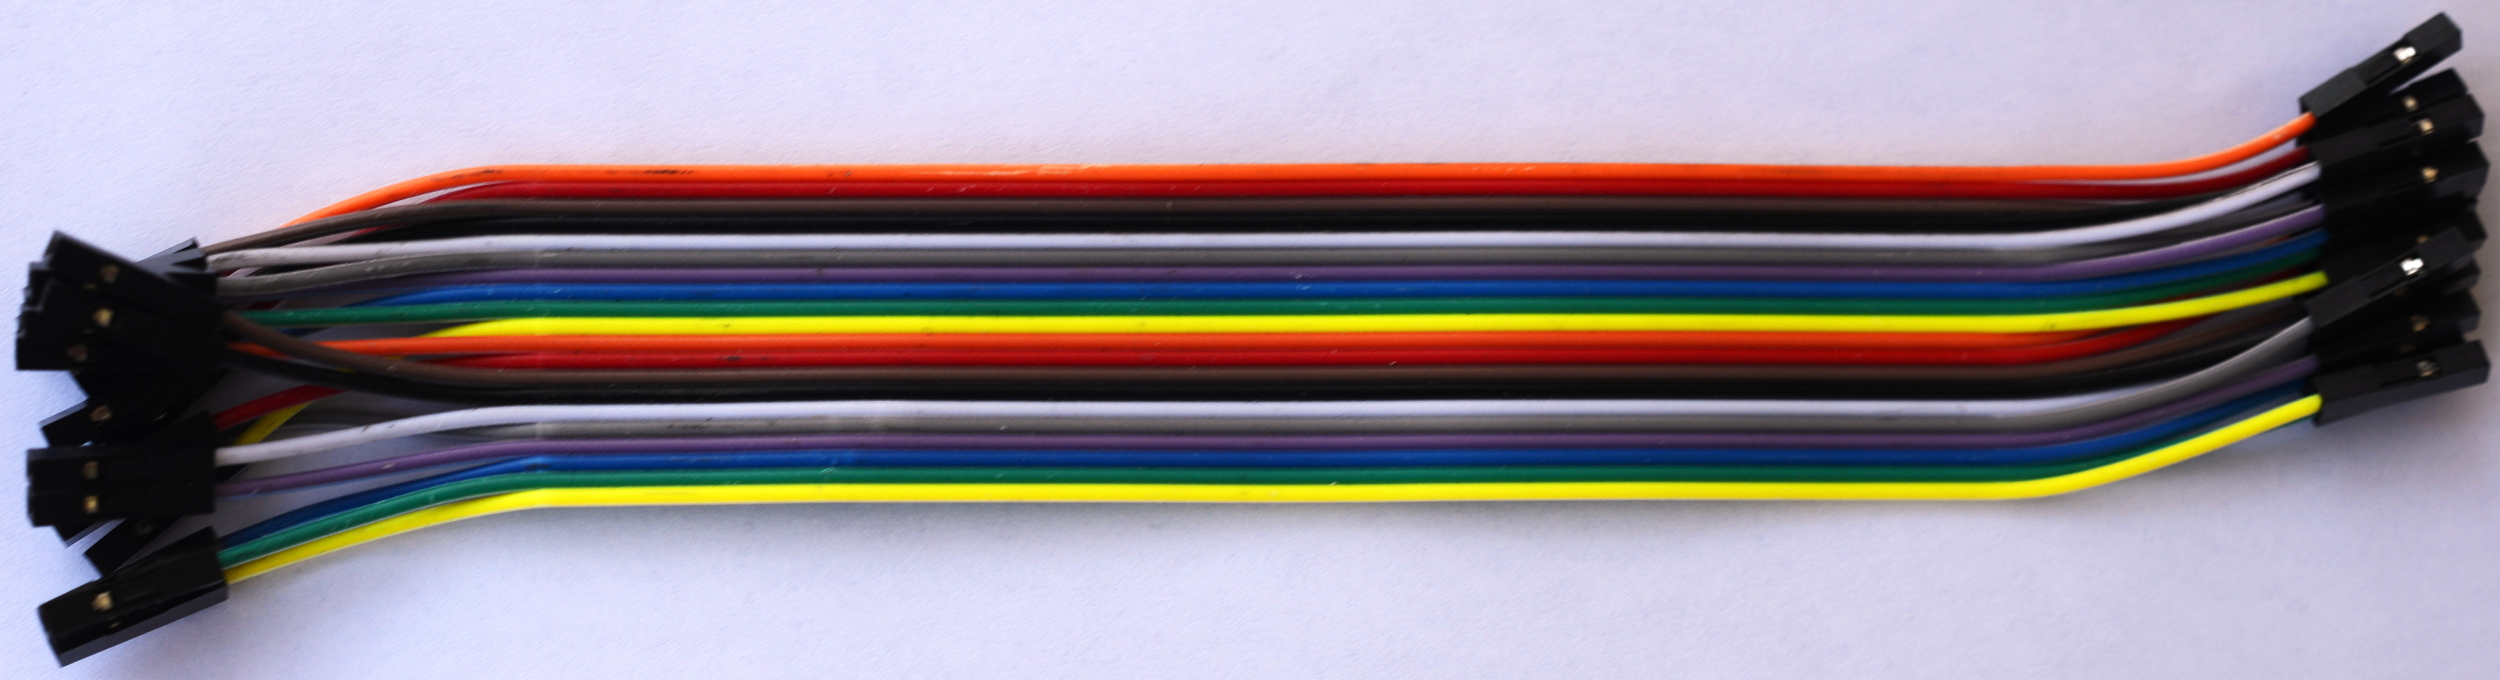
\includegraphics[width=0.49\textwidth]{images/sensor/cable_dupont.jpg}
\item Micro-USB-Kabel
\item Zugang zu Wifi-Netzwerk (ESSID + Passphrase), optional ein Freifunk-Router
\end{itemize}

% \newpage
% optionale Bauteile
% 
% \begin{itemize}
% \item BMP180 (Luftdruck) %, Temperatur(?), Feuchtigkeit(?))
% \item Display
% \item GPS \\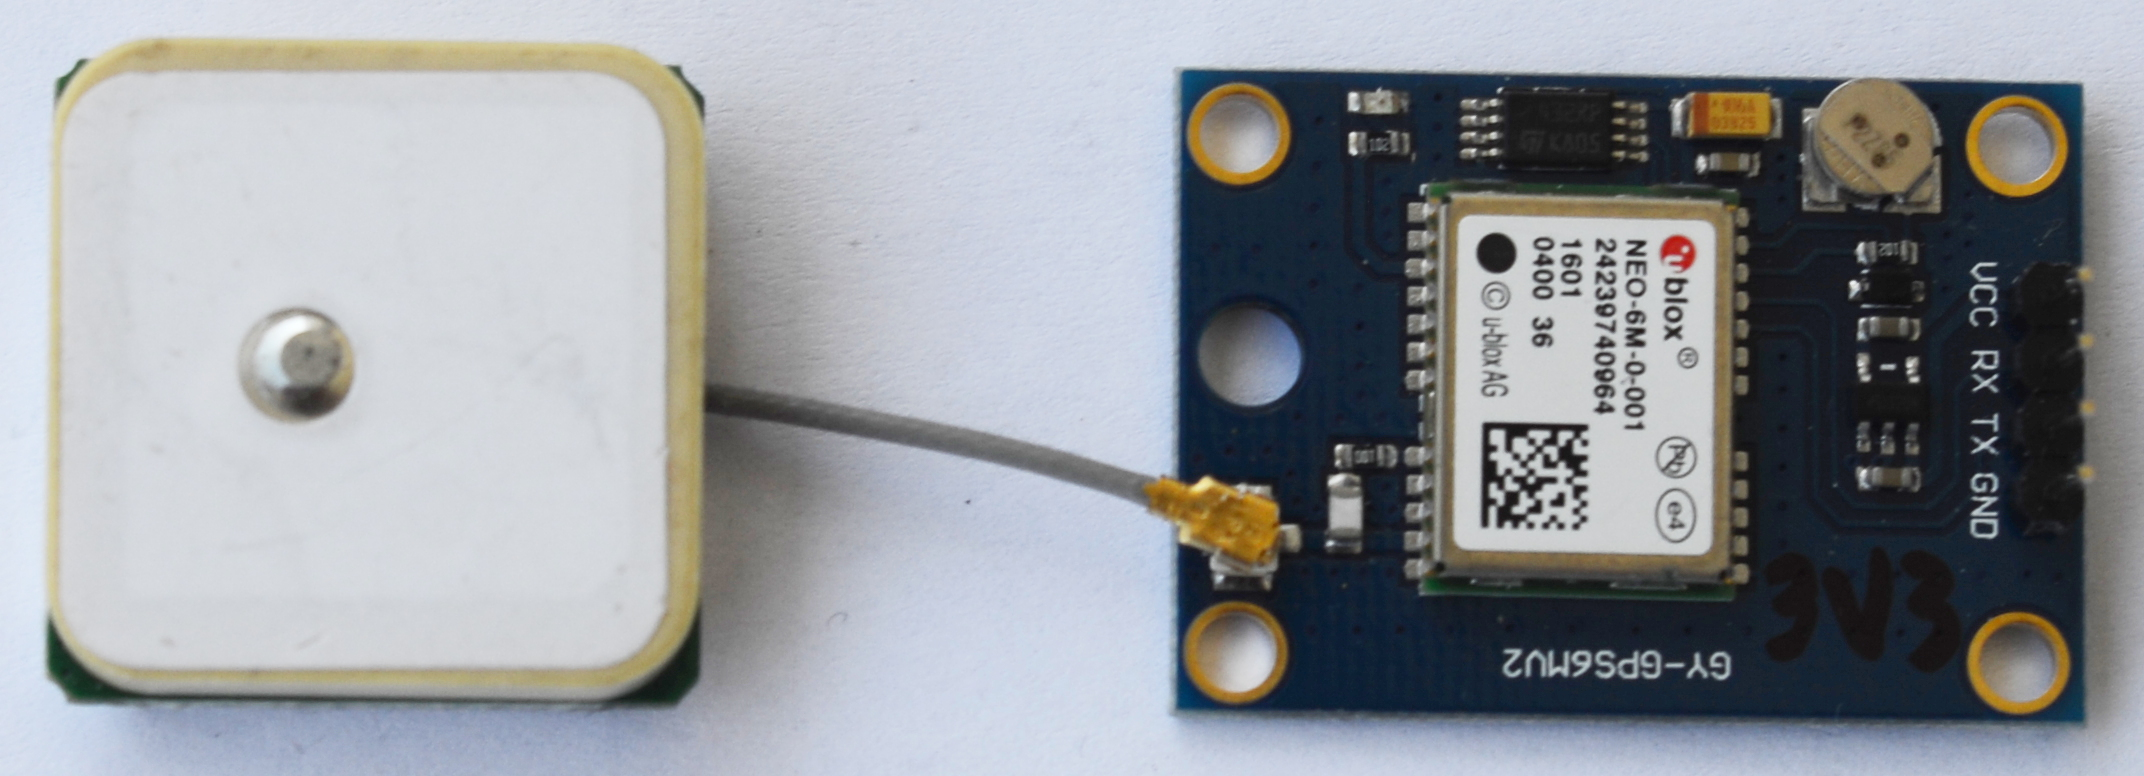
\includegraphics[width=0.49\textwidth]{images/sensor/gps.jpg}
% \end{itemize}

\section{Web}

\begin{description}

	\item[Homepage] \href{http://luftdaten.info/}{luftdaten.info}, \href{http://codefor.de/stuttgart/}{codefor.de/stuttgart}

	\item[Sourcecode] \href{https://github.com/opendata-stuttgart/}{github.com/opendata-stuttgart}
	%\begin{itemize}
		\\Wiki: \href{https://github.com/opendata-stuttgart/meta/wiki}{\dots/meta/wiki},
		Software: \href{https://github.com/opendata-stuttgart/sensors-software}{\dots/sensors-software},
	        BeginnersGuide: \href{https://github.com/opendata-stuttgart/sensors-software/blob/master/BeginnersGuide/Guide.md}{\dots/sensors-software/BeginnersGuide/}
	%\end{itemize}
	\item[Rohdaten] \href{http://archive.luftdaten.info/}{archive.luftdaten.info}
	\item[Plots] \href{https://www.madavi.de/sensor/graph.php}{www.madavi.de/sensor/graph.php}
	\item[Karte] \href{https://opendata-stuttgart.github.io/feinstaub-map/}{opendata-stuttgart.github.io/feinstaub-map}
	\item[Termine] \href{https://www.letsmeet.click/c/ok-lab-stuttgart/}{www.letsmeet.click/c/ok-lab-stuttgart}
		\\\href{http://www.meetup.com/de-DE/OK-Lab-Stuttgart-Meet-Up/}{www.meetup.com/de-DE/OK-Lab-Stuttgart-Meet-Up}%(Meetup, Termine)
\end{description}

% http://luftdaten.info/
% http://codefor.de/stuttgart/
% 
% https://github.com/opendata-stuttgart/
% https://github.com/opendata-stuttgart/meta/wiki
% https://github.com/opendata-stuttgart/sensors-software
% 
% http://archive.luftdaten.info/
% 
% http://www.meetup.com/de-DE/OK-Lab-Stuttgart-Meet-Up/
% https://www.letsmeet.click/c/ok-lab-stuttgart/

\end{document}
